\documentclass[10pt,a4paper,titlepage]{report}
\usepackage[latin1]{inputenc}
\usepackage{amsmath}
\usepackage{amsfonts}
\usepackage{amssymb}
\usepackage[labelfont=bf]{caption}
\usepackage{float}
\usepackage{listings}
\usepackage[section]{placeins}
\usepackage{graphicx}
\usepackage[left=2cm,right=2cm,top=2cm,bottom=2cm]{geometry}
\usepackage{tikz}
\author{Elijah Andrews}
\title{Implementing the Discrete Element Method with OpenCL for GPUs}
\begin{document}
\chapter*{Nomenclature}
\chapter*{Abstract}
\tableofcontents
\chapter{Introduction}
\section{Previous Work}
\section{Single Particle Motion in Fluids}
\label{sec:Single Particle Motion in Fluids}
\section{Project Goals}
\chapter{The Discrete Element Method}
The Discrete Element Method (DEM) is a numerical method for simulating how particles move and interact. The general principle is that individual particles of a medium are treated as separate rather than making continuum assumptions. This makes it a good method for modelling behaviours in granular materials such as sand or rocks. The DEM can be implemented with either soft or hard collision models. Soft models allow for overlap and treat collisions as sustained events whereas hard models treat collisions as an instantaneous event and model forces as an impulse. Soft collision models have broader applicability as they model sustained contact and multiple simultaneous collisions as well as some other complex phenomena\cite{softvshard}. For this reason a soft contact model has been chosen for this work.
\section{DEM Forces}
\label{sec:DEM Forces}
The Discrete Element Method can simulate a number of different forces using a variety of models. The merits of some of the most common models are discussed in Tuley\cite{tuley}. For this work the simplest force models have been chosen to reduce the overall complexity of the simulation.
\subsection{Normal Contact Force}
In a real elastic collision there will be some deformation of the particles. Calculating the deformation itself would be computationally expensive and would not be of interest in the study of particle population behaviours. The interaction can be modelled as a linear spring-dashpot arrangement where the overlap between the two particles is the compression of the spring. There is also damping based on the relative velocity in the normal direction. The force is thus described by equation \ref{eq:normal contact force} where $k_{e}$ is the collision stiffness, $\delta$ is the particle overlap, $\mathbf{\hat{n}}$ is the unit vector normal to the collision, $\eta$ is the damping coefficient, and $\mathbf{u}_{n}$ is the normal velocity.%TODO Make this clearer.
\begin{equation}
\mathbf{F}_{n} = k_{e} \delta \mathbf{\hat{n}} - \eta \mathbf{u}_{n}
\label{eq:normal contact force}
\end{equation}
\subsection{Tangential Contact Force}
The tangential contact force is the friction between two particle surfaces. There are two regimes of friction force, static and dynamic. In the static regime there is no tangential motion and the friction acts to stop motion. In the dynamic regime two surfaces are sliding across one another and the friction acts to arrest this motion. The static regime usually has a higher friction coefficient than the dynamic regime. The simplest and least computationally expensive model for friction is a 'complex friction model'. This calculates values for both of the regimes and applies the minimum of the two calculations.\cite{tuley}
\\\\The static regime friction force is calculated with equation \ref{eq:static friction} where $k_f$ is the friction stiffness, $\zeta$ is the tangential displacement, and $\mathbf{\hat{t}}$ is the unit vector tangential to the collision. 
\begin{equation}
\mathbf{F}_{t}^{static} = - k_{f} \zeta \mathbf{\hat{t}}
\label{eq:static friction}
\end{equation}
\\The dynamic regime friction force is calculated with equation \ref{eq:dynamic friction} where $\mu$ is the coefficient of friction.
\begin{equation}
\mathbf{F}_{t}^{dynamic} = - \mu |\mathbf{F}_{n}| \mathbf{\hat{t}}
\label{eq:dynamic friction}
\end{equation}
\\The final tangential friction force is defined in equation \ref{eq:friction force}.
\begin{equation}
\mathbf{F}_{t} = -\mathbf{\hat{t}}min(|\mathbf{F}_{t}^{static}|, |\mathbf{F}_{t}^{dynamic}|)
\label{eq:friction force}
\end{equation}
\subsection{Cohesion Force}
Cohesion is the attractive force between two bodies of the same material, adhesion is the attractive force between two bodies of different materials. For this work all of the particles and walls are assumed to be of the same material and so only cohesion is considered, however adhesion could be modelled with different constants. Although there are many complex effects that could be considered\cite{tuley}, a basic linear approximation can be used to model a cohesion force. This is defined in equation \ref{eq:cohesion force} where $k_c$ is the cohesion stiffness and $\delta_e$ is the particle effect surface overlap.
\begin{equation}
\mathbf{F}_{c} = k_{c} \delta_{e} \mathbf{\hat{n}}
\label{eq:cohesion force}
\end{equation}
\section{Equations of Motion}
The motion of particles in the simulation is governed by equation \ref{eq:acceleration}. This is derived from Newton's Second Law of motion. The total force, $\mathbf{F}$ is a combination of forces as shown in equation \ref{eq:total force}. $\mathbf{F}_{n}$, $\mathbf{F}_{t}$, and $\mathbf{F}_{c}$ are the forces defined in section \ref{sec:DEM Forces}. $\mathbf{F}_{g}$ and $\mathbf{F}_{d}$ are the gravitational force and drag force, respectively.
\\\textit{$<$These will be defined in section \ref{sec:Single Particle Motion in Fluids}$>$}.
\begin{equation}
\dfrac{du}{dt} = \dfrac{\mathbf{F}}{m}
\label{eq:acceleration}
\end{equation}
\begin{equation}
\mathbf{F} = \mathbf{F}_{n} + \mathbf{F}_{t} + \mathbf{F}_{c} + \mathbf{F}_{g} + \mathbf{F}_{d}
\label{eq:total force}
\end{equation}
Equation \ref{eq:acceleration} can be integrated twice to obtain the position of a particle at a time $t$.
\section{Rotation/Quaternions}
\textit{$<$This will be completed later as it is not immediately relevant to the progress of the project.$>$}
\section{Collision Detection}
It is most efficient to have the control volumes as small as possible because this reduces the number of particles in neighbouring control volumes. Control volumes must be at least as large as the largest particle to ensure that neighbouring control volumes contain all possible collisions. For monodisperse particle populations this means that the control volumes should be the same size as the particles. For polydisperse particle populations this means that the control volumes should be the size of the largest particle in the population. As mentioned in %TODO Reference
this can decrease efficiency for statistical distributions of particle sizes.
\chapter{Numerical Methods}
\section{Implicit/Explicit}

\section{Numerical Integration} \label{sec:Numerical Integration}
\subsection{Velocity}
Velocity is iterated with equation \ref{eq:particle_velocity_iteration} where $\dot{u}$ is the acceleration obtained from the function call 'Particle.get{\_}accel()'.
\begin{equation}
u_{n+1} = u_{n} + \dot{u} \Delta t
\label{eq:particle_velocity_iteration}
\end{equation}
\subsection{Position}
Position is iterated with equation \ref{eq:particle_position_iteration}.
\begin{equation}
x_{n+1} = x_{n} + \dfrac{u_{n+1} + u_{n}}{2}\Delta t 
\label{eq:particle_position_iteration}
\end{equation}
\subsection{Method of Integrating Drag}
There are three different methods of integrating drag. Firstly, there is the analytical solution, this is the exact solution to the model but cannot be done easily computationally. Secondly, there is the explicit numerical solution, this takes the current state and estimates the future state. Thirdly, there is the implicit numerical solution, this assumes the future state and integrates accordingly.
For a simple system with constant flow speed and no gravity, the system acceleration is described by equation \ref{eq:drag_acceleration}.
\begin{equation}
\dot{u} = \dfrac{v-u}{\tau}
\label{eq:drag_acceleration}
\end{equation}
Equation \ref{eq:drag_acceleration} can be solved to show that the analytical solution for the particle speed, $u$, is that in equation \ref{eq:analytical_drag_speed}.
\begin{equation}
u(t) = v(1 - e^{-\dfrac{t}{\tau}})
\label{eq:analytical_drag_speed}
\end{equation}
The explicit numerical integration method for equation \ref{eq:drag_acceleration} is that in equation \ref{eq:explicit_drag_speed}. Where $u_{n}$ is the current speed and $u_{n+1}$ is the speed after timestep $\Delta t$.
\begin{equation}
\dfrac{u_{n+1} - u_{n}}{\Delta t} = \dfrac{v - u_{n}}{\tau}
\label{eq:explicit_drag_speed}
\end{equation}
The implicit numerical integration method for equation \ref{eq:drag_acceleration} is that in equation \ref{eq:implicit_drag_speed}. Where $u_{n}$ is the current speed and $u_{n+1}$ is the speed after timestep $\Delta t$.
\begin{equation}
\dot{u} = \dfrac{u_{n+1} - u_{n}}{\Delta t} = \dfrac{v - u_{n+1}}{\tau}
\label{eq:implicit_drag_speed}
\end{equation}
Equation \ref{eq:implicit_drag_speed} can be rearranged to get an equation of the form $\dot{u} = f(u_{n})$ as shown in equation \ref{eq:implicit_drag_acceleration}.
\begin{equation}
\dot{u} = \dfrac{v - u_{n}}{\tau + \Delta t}
\label{eq:implicit_drag_acceleration}
\end{equation}
When these three methods are applied to the system they produce the results in figure \ref{fig:particle_speed_for_different_integrations}.
\begin{figure}[!ht]
\centering
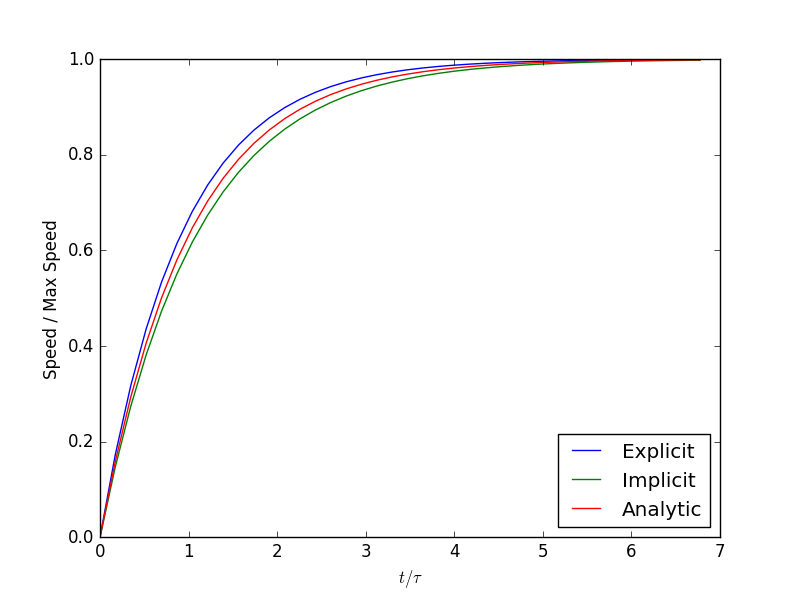
\includegraphics[scale=0.75]{figures/ParticleSpeedWithVaryingIntegration.png}
\caption{A graph of particle speed against time for the three methods of integration.}
\label{fig:particle_speed_for_different_integrations}
\end{figure}
\\Comparing the explicit and implicit numerical integration to the analytical solution shows that the explicit method has an average percentage difference of 2.05\% and the implicit method has an average percentage difference of 1.85\% when the timestep is $0.1 s$.
\\The average percentage difference can be compared between the two methods with varying timesteps as shown in figure \ref{fig:avg_percent_diff_against_timestep}. This graph shows that the explicit method increases its average percentage difference approximately linearly with increasing timestep. The implicit method increases its average percentage difference non-linearly at a slower rate than the explicit method. This implies that the implicit method is more accurate than the explicit method, especially for higher timesteps.
\begin{figure}[!htb]
\centering
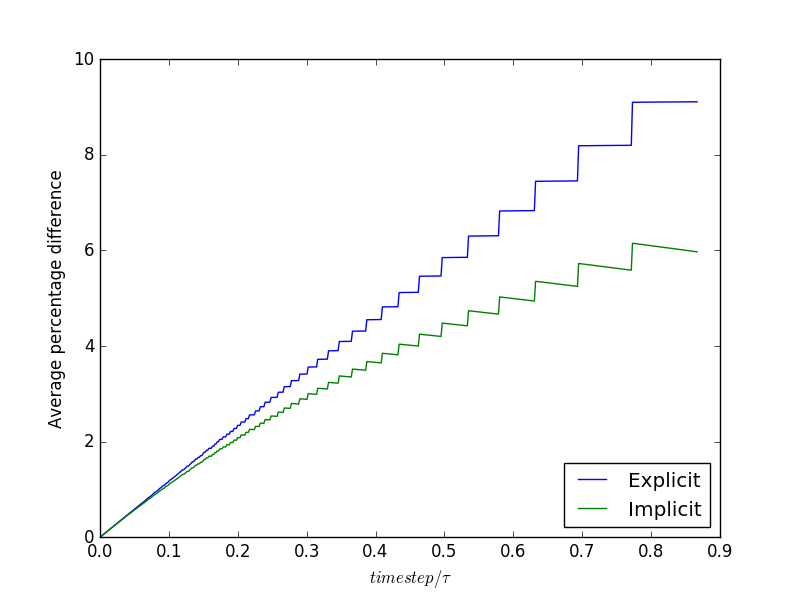
\includegraphics[scale=0.75]{figures/AveragePercentageDifferenceAgainstTimestep.png}
\caption{A graph of average percentage difference between the numerical method and analytical solution against varying timestep. The jaggedness of the lines is due to the discrete changes in timestep causing small rounding errors.}
\label{fig:avg_percent_diff_against_timestep}
\end{figure}
\\Unlike the explicit method, the implicit method depends on the other accelerations in the system. Equation \ref{eq:implicit_drag_acceleration} can be redefined to include these other accelerations as an extra $\dot{u}_{e}$ term as shown in equation \ref{eq:drag_acceleration_with_other_accelerations}.
\begin{equation}
\dot{u} = \dfrac{u_{n+1} - u_{n}}{\Delta t} = \dfrac{v - u_{n+1}}{\tau} + \dot{u}_{e}
\label{eq:drag_acceleration_with_other_accelerations}
\end{equation}
As before, equation \ref{eq:drag_acceleration_with_other_accelerations} can be rearranged to be in the form $\dot{u} = f(u_{n})$ as shown in equation \ref{eq:implicit_drag_acceleration_with_other_accelerations}. The derivation of this can be found in appendix \ref{sec:implicit_drag_accel_derivation}.
\begin{equation}
\dot{u} = \dfrac{v - u_{n} + \tau \dot{u}_{e}}{\tau + \Delta t}
\label{eq:implicit_drag_acceleration_with_other_accelerations}
\end{equation}
Equation \ref{eq:implicit_drag_acceleration_with_other_accelerations} can be applied to a particle falling under the effect of gravity through a stationary fluid. The results are shown in figure \ref{fig:fig:terminal_velocity_implicit_explicit}. As with the previous system, the explicit method has an average percentage difference of 2.05\% and the implicit method has an average percentage difference of 1.85\% when the timestep is $0.1 s$. This shows that the accuracy of the modified equation is consistent with that of equation \ref{eq:implicit_drag_acceleration}.
\begin{figure}[!htb]
\centering
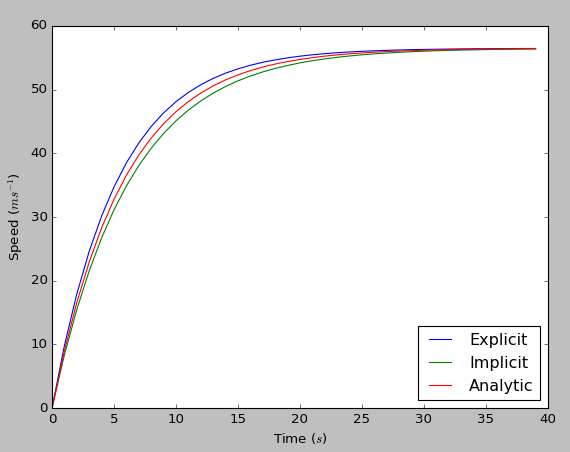
\includegraphics[scale=0.75]{figures/TerminalVelocityImplicitExplicit.png}
\caption{A graph of particle speed against time for each method of integration using equation \ref{eq:implicit_drag_acceleration_with_other_accelerations}.}
\label{fig:fig:terminal_velocity_implicit_explicit}
\end{figure}
\chapter{Python Implementation}
\section{Overview}
An initial implementation of the Discrete Element Method has been done in Python. The objective of this implementation is to gain an understanding of the DEM and any inherent computational difficulties. Python has been chosen as a testing environment for its simplicity and ease of development. 
\section{Element Types}
Different element types are required for different types of geometry and particle. For the Python implementation the two simplest have been chosen, a spherical particle and an axis-aligned wall.
\subsection{Particle}
The basic particle element is a spherical particle with pre-determined properties. These properties include initial position, initial velocity, diameter, density, fluid viscosity, and functions for fluid velocity and gravity. All of these properties can be set upon instantiation of each particle object and so can be easily modified for a variety of different simulations.
\\There are two objects for particles, the main object, 'Particle', tracks a full particle state history which is very memory intensive and unnecessary for most applications. The second object, 'LowMemParticle', inherits from 'Particle' and only keeps track of the current state and, during iteration, one future state.
\\The particle is iterated using the function call 'Particle.iterate()'. This passes a $\Delta t$ to the particle object and iterates the velocity and position. The methods used for integrating these properties are discussed in section \ref{sec:Numerical Integration}.
\subsection{Axis-Aligned Simple Wall}
The basic wall element is an axis-aligned simple wall. This object is defined by two points, minimum and maximum, that must lie in the same plane. From them a rectangle is formed. A normal is calculated for the wall and stored in the object to save time in collision calculations. The wall is treated as fixed, eliminating the need for complex material properties or calculation of motion.
\section{Collisions}
\subsection{Collision Detection}
Broad phase collision detection uses the simple spatial zoning technique described in Tuley\cite{tuley}. This approach has been chosen because it is quick and simple to implement. Other options were considered for this implementation but the benefits of using them were far outweighed by the complexity that using them would add to the overall algorithm. Since the initial Python implementation will not be fast anyway it was not deemed necessary to implement optimised algorithms at this stage.
\\The domain is represented by a three dimensional array where each entry is a control volume. The control volume is a list of particles in its bounds. The list of particles is iterated over and each particle assigns itself to the correct control volume. This results in a three dimensional array where each control volume has all of the particles within its bounds as an array. Collision objects are then created for each pair of particles in the same, or neighbouring, control volumes. This approach reduces the problem from $O(N^{2})$ to almost $O(N)$ as shown in figure \ref{fig:run_time_against_N_python}.
\begin{figure}[!ht]
\centering
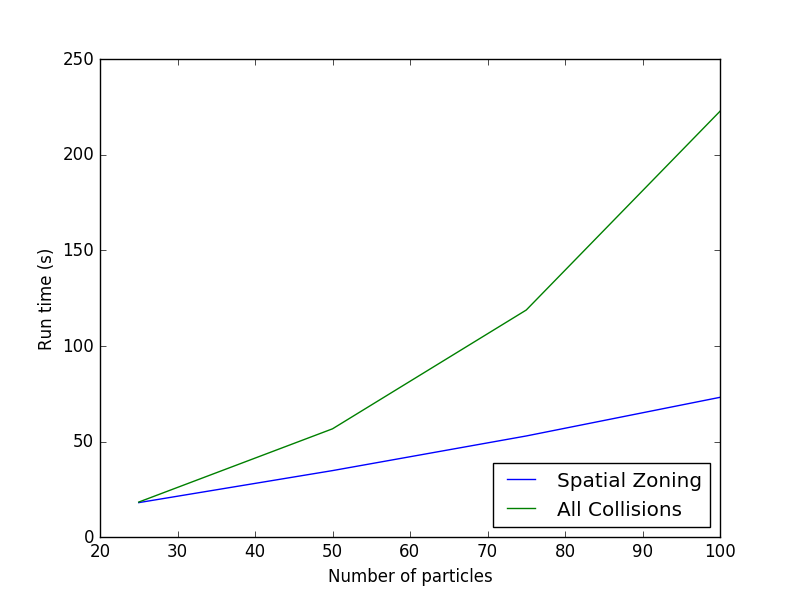
\includegraphics[scale=0.75]{figures/RunTimeAgainstNumberOfParticlesPython.png}
\caption{This graph shows that the simple spatial zoning technique reduces the problem from $O(N^{2})$ down to almost $O(N)$.}
\label{fig:run_time_against_N_python}
\end{figure}
\subsection{Collision Resolution}
After an array of collisions has been generated they are iterated over and each collision is resolved. First, the distance between particles is calculated to determine if they are in contact. Often this reveals that they are not in contact and the calculation ends there. If particles are in contact then collision forces are determined.
\\In this initial Python implementation only the simple normal and tangential contact forces are calculated. These are enough to run sufficient initial test cases.
\section{Calculating Forces}
There are three categories of forces used in this implementation. These are drag (particle-fluid interaction), gravity, and DEM forces.
\subsection{Drag}
The drag forces are determined using Stokes' law as discussed in %TODO Reference
This is calculated using a flow field calculation function that is passed into the Particle object upon instantiation. The particle then calls this function as part of its get\_accel() function. This allows a variety of flow field functions to be used without modifying the Particle object code. The default for this function is a perfectly stationary flow.
\subsection{Gravity}
Gravity is treated in a similar manner to drag. A gravity function can be passed into the Particle object upon instantiation. Although this defaults to a simple -9.81$ms^{-1}$, it can be chosen to simulate a rotating frame of reference or other complex configurations. A rotating frame of reference has been implemented in the ``gravity\_shift\_closed\_box'' example simulation. %TODO Reference github
\subsection{DEM Forces}
The DEM forces that are calculated in collisions are stored in an array within the Particle object. When the particle is iterated the array is added together and used in the integration calculation. After this calculation the array is cleared so that forces don't get incorrectly added multiple times. This configuration makes it simple to add and remove forces to the simulation whenever necessary and could also be used in general to add any force to the particle.
\section{Verification}
To asses the accuracy of the implementation a series of cases have been tested and compared to analytical solutions of the model.
\subsection{Settling Overlap}
In this case two particles are used. The first particle is an ordinary particle acting under the effects of gravity. The second particle, placed below the first particle, is a particle with quasi-infinite density without being affected by gravity. As time increases the first particle bounces on the second particle until it eventually comes to rest with some overlap with the second particle.\\
\begin{figure}[!htb]
\centering
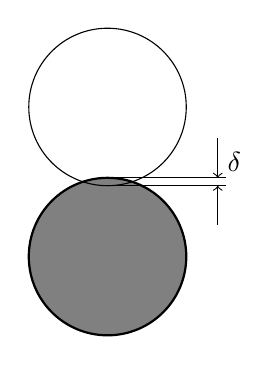
\begin{tikzpicture}
\filldraw[color=black, fill=gray, thick] circle (1);
\draw  (0, 1.9) circle (1);
\draw (0, 1) -- (1.5, 1);
\draw (0, 0.9) -- (1.5, 0.9);
\draw[->] (1.4, 1.5) -- (1.4, 1);
\draw[->] (1.4, 0.4) -- (1.4, 0.9);
\filldraw[black] (1.4, 1.2) node[anchor=west] {$\delta$};
\end{tikzpicture}
\caption{A particle, under the effect of gravity, resting upon a second particle of infinite density, unaffected by gravity. Overlap, $\delta$, is labelled and exaggerated for clarity.}
\end{figure}
\\For the particle to be at rest the particle's gravity must be equal to the normal force from the DEM.
\begin{equation}
F_{g} = F_{n}
\end{equation}
\begin{equation}
mg = k_{e}\delta - \eta u
\end{equation}
To get an equation for overlap, $\delta$, the equation is simplified and rearranged. The speed, $u$, is 0 at rest.
\begin{equation}
\delta = \dfrac{mg}{k_{e}}
\end{equation} 
Taking particle diameter to be 0.1 $m$ and particle density to be 2000 $kg m^{-3}$, the particle mass is 1.047 $kg$. Gravity is taken to be 9.81 $m s^{-2}$ and model spring stiffness is $10^{5}$.
\begin{equation}
\delta = \dfrac{1.047 * 9.81}{10^{5}} = 1.027 * 10^{-4}
\end{equation} 
Running a simulation with these parameters also yields an overlap of $1.027 * 10^{-4}$. Comparing simulation results with high precision overlap prediction shows that the simulation result is within $2.1 * 10^{-11}\%$ of the predicted value.
\subsubsection{Timestep stability}
This result can also be compared for varying timesteps to asses the stability of the implementation. Figure \ref{fig:overlap_percentage_error_against_timestep} shows very stable results up until a timestep of approximately 0.00097.
\begin{figure}[!htb]
\chapter{OpenCL and Graphics Processing Units}
\centering
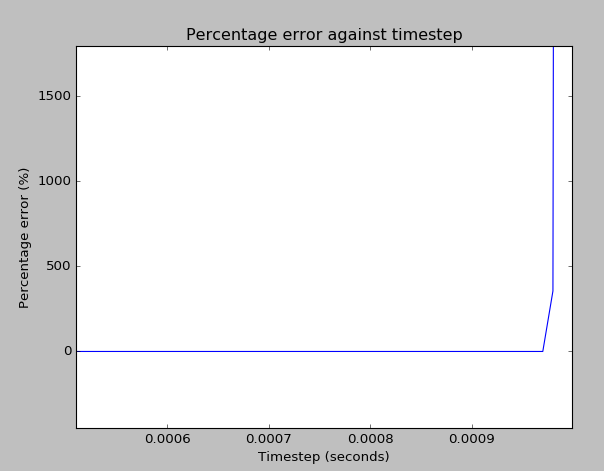
\includegraphics[scale=0.75]{figures/ParticleBounceTimestepAgainstPercentageError.png}
\caption{A graph of overlap percentage error against time step.}
\label{fig:overlap_percentage_error_against_timestep}
\end{figure}
\subsection{Timestep Stability}
Collisions go boom if timestep is too high etc. %<Test against bouncing or something>
The stiffer the collisions the smaller the timestep must be to maintain physical results.
This can be spotted and logged if $E_{k}$ is higher after collision than before.
%TODO Run a simulation of timestep against stiffness.
\chapter{OpenCL Implementation}
\section{Data Structures}
As the C language does not support objects, the objects used in the Python implementation must be simplified into data structures and separate functions. Most of the calculations that were done in the object functions will now be done within the kernels.
\subsection{Particle}
The particle structure contains very similar information as the Python implementation particle object. Notable differences are the lack of 'next\_$<$property$>$' variables since these are just used within the iterate\_particle kernel and do not need to be stored.
\\The structure is aligned to the nearest 128 bytes of memory to make accessing it easier. This does waste a little under half of this memory but for $10^7$ particles the particle array requires a total of 1.2GB which is within workable limits.
\subsection{Collision}
The collision structure contains two particle IDs and collision properties. This could be reduced to just particle IDs if collisions were taken as having the same properties throughout the simulation. Alternatively, if the collision changed based on particle properties, the collision resolution kernel could calculate the collision properties when they are needed.
\subsection{Buffers}
To access the data from the device it must be passed into a buffer. None of the structure data is passed into the buffer so the device must have the same definition of the structure as the host. This is problematic as the host and device have different compilers. To work around this problem the host and device structures are written with members in descending order of size. In addition padding has been added to the host code %TODO Make sure this is the case
 since the alignment specifier is apparently insufficient to ensure correct alignment. The alignment attribute specifier is also not the same between different compilers so ``if defined'' statements are implemented for both Visual Studio and GCC compilers. The code for these definitions is shown in figure \ref{fig:struct_definitions}.

\begin{figure}[!ht]
Host:
\begin{lstlisting}[language=C]
typedef struct {
    cl_float3 pos;
    cl_float3 vel;
    cl_float3 forces;
    cl_ulong particle_id;
    cl_float particle_diameter;
    cl_float density;
    cl_float fluid_viscosity;
    cl_char padding[56];
// Structure memory alignment for Visual Studio and GCC compilers.
#if defined(_MSC_VER)
} __declspec(align(128)) particle;
#elif defined(__GNUC) || defined(__GNUG__)
} __attribute__((aligned (128))) particle;
#endif
\end{lstlisting}
Device:
\begin{lstlisting}[language=C]
typedef struct {
    float3 pos;
    float3 vel;
    float3 forces;
    ulong particle_id;
    float particle_diameter;
    float density;
    float fluid_viscosity;
} __attribute__ ((aligned (128))) particle;
\end{lstlisting}
\caption{Host and device definitions of the particle structure.}
\label{fig:struct_definitions}
\end{figure}
\section{Kernels}
The main calculations for this implementation are performed on the device. This means that the program must be separated into kernels to be passed over sets of data.
\subsection{Collision Detection}
To improve efficiency, in both speed and resource usage, performing naive collision detection is not viable for large numbers of particles. To improve on this the spatial zoning technique is used similar to the initial Python implementation. However, C does not make arrays of varying sizes easy or efficient so the data structures used and the algorithm implementation must be significantly different.
\\The basic problem is how to store control volumes as lists of references to particles. In Python this was easy, a simple 3D array of control volumes with lists of particle objects inside was sufficient. Various approaches to solving this problem were considered. One approach was to encode particle IDs (equal to the index of a particle in the particles array) with a hashing function into a single number that could be turned back into particle IDs on the device. However, this approach was infeasible because the numbers would get so large that they could not be stored accurately or efficiently.
\\The approach used is to have multiple passes of assignment of particles to control volumes. The first pass simply counts how many particles are in each control volume. This is stored in a single dimensional array of control volumes represented by integers of how many particles each contains. From this array another array is created. This array is of all the particle IDs but sorted into control volumes. The control volumes are of lengths defined by the count array and start at indexes stored in a third array. If a control volume has no particles, the start index of the array is set to -1. For the unsigned long data type this overflows to the maximum value (approximately 4.3 billion) which will likely never be used to index particles. When creating collisions this assumption will be checked and a warning issued. This arrangement of arrays is shown in figure \ref{fig:cv_array_structure}.
\\This approach is somewhat similar to how memory is handled on a computer, but using indexes instead of pointers. For an entirely host-side method an array of pointers to arrays of particles could be used, but this would not be sensible when dealing with device memory as each array would need to be moved to the device before use. Having three arrays that hold all the necessary properties simplifies the memory buffer process significantly. The maths required for turning positions and control volume coordinates into indexes in these arrays are contained in cvUtils.c and kernelUtils.cl for host and device, respectively.
\begin{figure}[!ht]
\usetikzlibrary{patterns}
\begin{tikzpicture}


\draw [pattern=horizontal lines][help lines, step=1cm] (-5,-1) node (v19) {} grid (4,0) node (v60) {};

\node (v20) at (-4.5,-0.5) {4};
\node (v21) at (-3.5,-0.5) {2};
\node at (-2.5,-0.5) {0};
\node at (-1.5,-0.5) {0};
\node at (-0.5,-0.5) {3};
\node at (0.5,-0.5) {5};
\node at (1.5,-0.5) {3};
\node at (2.5,-0.5) {2};
\node at (3.5,-0.5) {1};

\draw [pattern=horizontal lines][help lines, step=1cm] (-5,-3) node (v1) {} grid (4,-2) node (v40) {};

\node at (-4.5,-2.5) {0};
\node at (-3.5,-2.5) {4};
\node at (-2.5,-2.5) {-1};
\node at (-1.5,-2.5) {-1};
\node at (-0.5,-2.5) {6};
\node at (0.5,-2.5) {9};
\node at (1.5,-2.5) {14};
\node at (2.5,-2.5) {17};
\node at (3.5,-2.5) {19};

\draw [pattern=horizontal lines][help lines, step=0.5cm] (-5.5,-4.5) grid (4.5,-4) node (v18) {};


\node (v2) at (-5.5,-4) {};
\node at (-5,-4) {};
\node at (-4.5,-4) {};
\node at (-4,-4) {};
\node (v4) at (-3.5,-4) {};
\node at (-3,-4) {};
\node (v6) at (-2.5,-4) {};
\node at (-2,-4) {};
\node at (-1.5,-4) {};
\node (v10) at (-1,-4) {};
\node at (-0.5,-4) {};
\node at (0,-4) {};
\node at (0.5,-4) {};
\node at (1,-4) {};
\node (v12) at (1.5,-4) {};
\node at (2,-4) {};
\node at (2.5,-4) {};
\node (v14) at (3,-4) {};
\node at (3.5,-4) {};
\node (v16) at (4,-4) {};

\node (v3) at (-4,-3) {};
\node (v5) at (-3,-3) {};
\node (v7) at (-2,-3) {};
\node (v8) at (-1,-3) {};
\node (v9) at (0,-3) {};
\node (v11) at (1,-3) {};
\node (v13) at (2,-3) {};
\node (v15) at (3,-3) {};
\node (v17) at (4,-3) {};

\draw  (v2) rectangle (-3.5,-4.5);
\draw  (v4) rectangle (-2.5,-4.5);
\draw  (v6) rectangle (-1,-4.5);
\draw  (v10) rectangle (1.5,-4.5);
\draw  (v12) rectangle (3,-4.5);
\draw  (v14) rectangle (4,-4.5);
\draw  (v16) rectangle (4.5,-4.5);
\node (v22) at (-5,-2) {};
\node (v24) at (-4,-2) {};
\node (v26) at (-3,-2) {};
\node (v28) at (-2,-2) {};
\node (v30) at (-1,-2) {};
\node (v32) at (0,-2) {};
\node (v34) at (1,-2) {};
\node (v36) at (2,-2) {};
\node (v38) at (3,-2) {};
\node (v23) at (-4,-1) {};
\node (v25) at (-3,-1) {};
\node (v27) at (-2,-1) {};
\node (v29) at (-1,-1) {};
\node (v31) at (0,-1) {};
\node (v33) at (1,-1) {};
\node (v35) at (2,-1) {};

\node (v39) at (4,-1) {};
\node (v37) at (3,-1) {};

\node at (-7.5,-0.5) {Particle Count Array};
\node at (-7.5,-2.5) {CV Start Index Array};
\node at (-7.5,-4.25) {Sorted Particle Array};



\draw [dashed] (v19) edge (v22);
\draw [dashed] (v23) edge (v24);
\draw [dashed] (v25) edge (v26);
\draw [dashed] (v27) edge (v28);
\draw [dashed] (v29) edge (v30);
\draw [dashed] (v31) edge (v32);
\draw [dashed] (v33) edge (v34);
\draw [dashed] (v35) edge (v36);
\draw [dashed] (v37) edge (v38);
\draw [dashed] (v39) edge (v40);
\draw [dashed] (v1) edge (v2);
\draw [dashed] (v3) edge (v4);
\draw [dashed] (v5) edge (v6);
\draw [dashed] (v7) edge (v6);
\draw [dashed] (v8) edge (v6);
\draw [dashed] (v9) edge (v10);
\draw [dashed] (v11) edge (v12);
\draw [dashed] (v14) edge (v13);
\draw [dashed] (v15) edge (v16);
\draw [dashed] (v17) edge (v18);

\draw [help lines, step=1cm] (-5,1) node (v41) {} grid (4,2);
\node at (-4.5,1.5) {0};
\node at (-3.5,1.5) {1};
\node at (-2.5,1.5) {2};
\node at (-1.5,1.5) {3};
\node at (-0.5,1.5) {4};
\node at (0.5,1.5) {5};
\node at (1.5,1.5) {6};
\node at (2.5,1.5) {7};
\node at (3.5,1.5) {8};
\node (v42) at (-5,0) {};
\node (v44) at (-4,0) {};
\node (v46) at (-3,0) {};
\node (v48) at (-2,0) {};
\node (v50) at (-1,0) {};
\node (v52) at (0,0) {};
\node (v56) at (1,0) {};

\node (v58) at (3,0) {};
\node (v54) at (2,0) {};
\node (v43) at (-4,1) {};
\node (v45) at (-3,1) {};
\node (v47) at (-2,1) {};
\node (v49) at (-1,1) {};
\node (v51) at (0,1) {};
\node (v55) at (1,1) {};
\node (v53) at (2,1) {};
\node (v57) at (3,1) {};
\node (v59) at (4,1) {};
\draw [dashed] (v41) edge (v42);
\draw [dashed] (v43) edge (v44);
\draw [dashed] (v45) edge (v46);
\draw [dashed] (v47) edge (v48);
\draw [dashed] (v49) edge (v50);
\draw [dashed] (v51) edge (v52);
\draw [dashed] (v53) edge (v54);
\draw [dashed] (v55) edge (v56);
\draw [dashed] (v57) edge (v58);
\draw [dashed] (v59) edge (v60);
\node at (-7.5,1.5) {CV Index};
\end{tikzpicture}
\caption{Diagram showing the structure and relationship between arrays representing Control Volumes.}
\label{fig:cv_array_structure}
\end{figure}
\\One weakness of this approach is that the CV start index array is generated sequentially. A solution to this weakness could be to have each control volume add up the number of particles in all preceding control volumes in order to determine its own start index in the sorted particle array. However, this would repeat a lot of maths and could end up being slower. The function consists of adding to the start index count and then assigning the count to memory in the CV start index array. If it were to be done in parallel, the adding would have to be repeated for each CV but the memory assignment would be done in parallel. Thus, whether it would be faster sequentially or in parallel depends on which operation is slower. This [could be]/[is] benchmarked in a later part of this project. %TODO benchmark this. 

\subsection{Collision Resolution}
\label{sec:Collision Resolution}
The collision resolution kernel is actually separated into multiple kernels for different types of collision (particle-particle and particle-wall) however the behaviour of these kernels is almost identical. For this discussion we will use the particle-particle kernel as an example. The kernel takes a pointer to an array of collision structures and a pointer to the array of particles. The DEM collision force calculations are run for each collision and the forces are added to the DEM forces vector in the relevant particle structures. This approach has been chosen because it is easier to sum the forces as they are calculated rather than attempt to predict the length of the necessary force array to store each force separately as in the Python implementation.
\\This approach causes a serious problem as it is possible that multiple collision kernels will need to write data to the same particle at the same time. The solution to this is to use the atomic operations available in OpenCL. Unfortunately, OpenCL only natively supports full atomic operations for int and unsigned int data types. OpenCL does support an exchange atomic operator for single precision floats, but this is not the best approach for doing atomic arithmetic for floats.
\\An approach for doing atomic addition (as is necessary in this case) is presented in %TODO Reference website
The code is shown in figure \ref{fig:atomic_float_addition}. This approach uses the comparison exchange atomic operator by creating a union of the floats with unsigned ints. This works well because the bits being exchanged are the same for the float and unsigned int and actual atomic arithmetic is not necessary so the difference between the data types doesn't matter. Thus the new value is calculated and if the value used to calculate it has changed in that time the calculation is repeated with the updated value.
\begin{figure}[!ht]
\begin{lstlisting}[language=C]
 _INLINE_ void atomicAdd_g_f(volatile __global float *addr, float val)
   {
       union{
           unsigned int u32;
           float        f32;
       } next, expected, current;
   	current.f32    = *addr;
       do{
   	   expected.f32 = current.f32;
           next.f32     = expected.f32 + val;
   		current.u32  = atomic_cmpxchg( (volatile __global unsigned int *)addr, 
                               expected.u32, next.u32);
       } while( current.u32 != expected.u32 );
   }
\end{lstlisting}
\caption{Kernel code for a solution to atomic addition with floats.}
\label{fig:atomic_float_addition}
\end{figure}
\subsection{Particle Iteration}
Particle iteration is performed almost identically to the Python implementation. The implicit integration scheme, as outlined in section \ref{sec:Numerical Integration}, is used. The main difference, as discussed in section \ref{sec:Collision Resolution}, is that the OpenCL implementation performs the summation of DEM forces as they are calculated in collisions whereas the Python implementation performs the summation when iterating the particle.
\section{Unit Tests}
Due to the large size of the project and algorithmic complexity, it is important to test each unit of code individually rather than trying to trace bugs through the whole code-base. In addition, this project is intended to be run on heterogeneous devices and so differences in runtime environment could cause problems. For these reasons a unit testing approach has been chosen so that tests can be quickly re-run to check code unit functionality without assuming identical behaviour between systems.
\\Some functions are not included in the unit testing system due to their simplicity and the relatively long time it would take to program unit tests for all of them. For example, checking that a function multiplies numbers correctly does not need to be tested every time.
\subsection{Testing Framework}
Often a framework is used for unit testing, however there isn't a quick, easy framework available for C with OpenCL so a simple system has been set up to make running tests easy.
\\Each tested feature has a directory within the 'tests' directory with its header and C code files. A feature may have multiple functions, each with its own testing function. Each testing function takes a boolean paramter, 'verbose', that determines whether it prints intermediate results and debugging outputs. The functions return a boolean that indicates whether the test passed or not. In some cases, if a function fails, it may not be obvious why and so debugging outputs will be printed. For example, test\_assign\_particle\_count could have the wrong number of control volumes or incorrectly assigned particles so both of these outcomes has its own printed debugging output. %TODO Reference code
\\To make it easy to run these tests repeatedly 'run\_tests.c' has been created to run all of the tests and indicate which, if any, fails. A similar implementation can be executed at runtime from a simulation to ensure that all tests are passed before starting a simulation run.
\chapter{Results}
\section{Comparison between CPU and GPU}
\chapter{Application}
Modelling agglomerates...
\section{Modified Particle Structure}
Including effect diameter...
\section{Fluid Velocity Field}
get\_vel\_fluid... Taylor-Green Vortex...
\section{Results}
Pretty pictures etc...
\chapter{Conclusion}
\section{Further Work}
\appendix
\chapter{Derivations}
\section{Equation \ref{eq:implicit_drag_acceleration_with_other_accelerations}}
\label{sec:implicit_drag_accel_derivation}
\begin{align}
\dot{u} &= \dfrac{v - u}{\tau} + \dot{u}_{e}
\\\dfrac{u_{n+1} - u_{n}}{\Delta t} &= \dfrac{v - u_{n+1}}{\tau} + \dot{u}_{e}
\\u_{n+1} &= \dfrac{\dfrac{v}{\tau} + \dfrac{u_{n}}{\Delta t} + \dot{u}_{e}}{\dfrac{1}{\Delta t} + \dfrac{1}{\tau}}
\\\dfrac{u_{n+1} - u_{n}}{\Delta t} &= \dfrac{\Bigg(\dfrac{\dfrac{v}{\tau} + \dfrac{u_{n}}{\Delta t} + \dot{u}_{e}}{\dfrac{1}{\Delta t} + \dfrac{1}{\tau}}\Bigg) - u_{n}}{\Delta t}
\\\dot{u} &= \dfrac{v - u_{n} + \tau \dot{u}_{e}}{\tau + \Delta t}
\end{align}
\bibliography{references}
\bibliographystyle{unsrt}
\end{document}
